\section{Conclusion}~\label{sec.Conclusion}

In this section, we compare efficiency of the
\begin{enumerate}
    \item \textit{predictor 1: machine learning predictor}.
    \item \textit{predictor 2: theory time complexity predictor}.
    \item \textit{predictor 3: average running time}.
\end{enumerate}
to solve new generated graphs.

We will analysis the result and provide the further project focus.

\begin{figure}[h!]
    \centering
    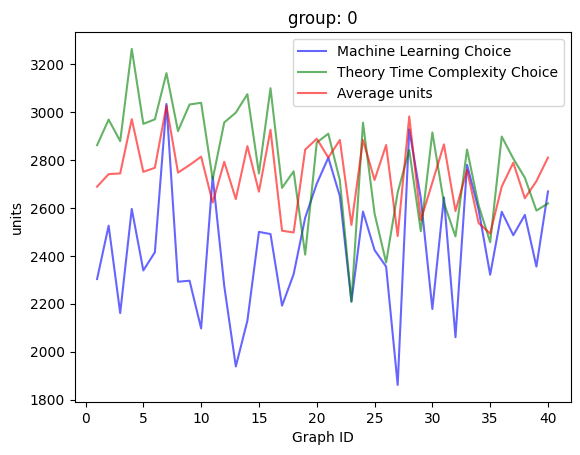
\includegraphics[width=0.36\textwidth]{result-1.png}
    \caption{combine tree-width, straight polynomial linear regression for run time}
    \label{combine tree-width, straight polynomial linear regression for run time}
    \end{figure}

The \textit{predictor 1} shows a very high performance averagely. That only cost 87.4\% run time of \textit{predictor 2} and 91.0\% run time of \textit{predictor 3}.

However, here is 2\% for this predictor that get huge differences, that the predicted run time is 2 times larger than real run time. Also, we found that the optimization is not so well when the tree width is large, and the efficiency smaller than related works.

We thought that, still the predictor has not sufficient data to do learning, especially in the large tree width area. Also, we found that our tree decomposition algorithm is a kind of combined algorithm, so that it is not uniformly random and will have a higher probability to already optimized tree decomposition.

Thus we may improve our project by constantly adding data and improve the basic algorithm parts.